\chapter{FPGA}

\section{Introducción}

Las FPGAs son dispositivos semiconductores que puede ser programados después de
la fabricación. En lugar de limitarse a una función predeterminada los FPGAs
pueden adaptarse a nuevas normas, y reconfigurar el hardware para
aplicaciones específicas, incluso después de que el producto ha sido instalado.

Es posible utilizar un FPGA para implementar cualquier función lógica a
un circuito integrado y tienen la capacidad de actualizar la funcionalidad
después de la primera configuración  por lo cual ofrece ventajas para muchas
aplicaciones.

Las FPGAs actuales consisten en varias combinaciones de SRAM integrada
configurable, transmisores-receptores de alta velocidad, alta velocidad de E/S,
bloques lógicos y enrutamiento de paquetes\cite{fpga}.

\begin{figure}[h!] 
 \centering
 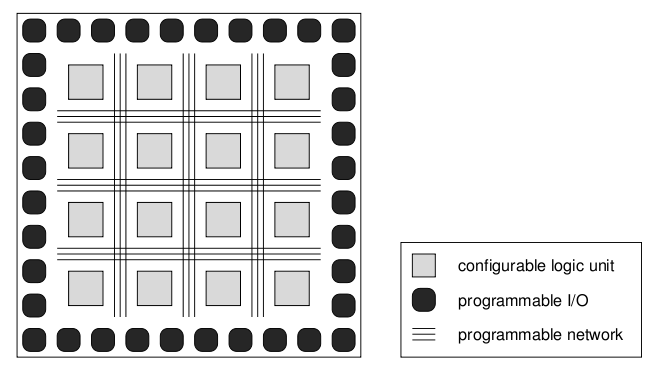
\includegraphics[scale=.50]{./figuras/Fpga.png}
 % capas.png: 607x522 pixel, 72dpi, 21.41x18.41 cm, bb=0 0 607 522
 \caption{FPGA genérico}
 \label{Tarjeta de desarrollo NetFPGA}
\end{figure}



Como uno de los más versátiles componentes de la tecnología VLSI\footnote{VLSI,
es el acrónimo \emph{Very Large Scale Integration}, integración en escala
muy grande. La integración en escala muy grande de sistemas de circuitos basados
en transistores en circuitos integrados comenzó en los años 1980, como parte de
las tecnologías de semiconductores y comunicación que se estaban
desarrollando.}, permite implementar complejos dispositivos electrónicos
diseñados mediante lenguajes de descripción de hardware como VHDL\footnote{VHDL,
es el acrónimo que representa la combinación de VHSIC y HDL, donde VHSIC es el
acrónimo de \emph{Very High Speed Integrated Circuit} y HDL es a su vez el
acrónimo de \emph{Hardware Description Language}.} o Verilog\footnote{Verilog es
un lenguaje de descripción de hardware usado para modelar sistemas electrónicos.
El lenguaje, algunas veces llamado \emph{Verilog HDL}, soporta el diseño, prueba
e implementación de circuitos analógicos, digitales y de señal mixta a
diferentes niveles de abstracción.}, además muchos de estos también contienen
dentro de sí diversos elementos como unidades de memoria que van desde simples
\emph{flip-flops} hasta bloques de memoria dinámica más complejos. También
pueden contener multiplicadores, comparadores e incluso procesadores para formar
sistemas programables en chips\cite{nava}.

% 
\section{NetFPGA}

El Proyecto NetFPGA se refiere a un esfuerzo para desarrollar un hardware de
código abierto y la plataforma de software que permite la rápida creación de
prototipos de dispositivos de red. 

NetFPGA se distingue principalmente en dos formas. En primer lugar se encuentra
en su enfoque basado en FPGA para dispositivos de red de creación de prototipos.
Esto permite a los usuarios desarrollar diseños que son capaces de procesar los
paquetes a velocidad de línea, una capacidad general no lograda por los
enfoques basados en \emph{software}. La segunda característica distintiva en el 
NetFPGA es su enfoque en el apoyo a una comunidad de \emph{hardware} de código
abierto y desarrolladores de \emph{software} que puedan compartir y construir
sobre cada uno de los proyectos y los bloques de construcción\cite{netfpga1}.

\begin{figure}[ht]
 \centering
 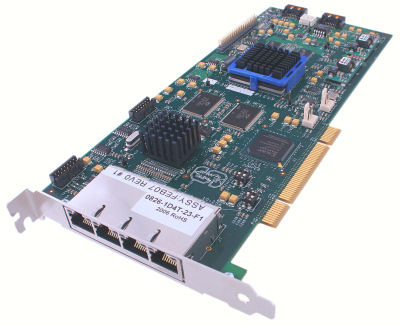
\includegraphics[scale=.50]{./figuras/netfpga.jpg}
 % capas.png: 607x522 pixel, 72dpi, 21.41x18.41 cm, bb=0 0 607 522
 \caption{Tarjeta de desarrollo NetFPGA}
 \label{Tarjeta de desarrollo NetFPGA}
\end{figure}


El NetFPGA incluye el todos los recursos de la lógica, la memoria, y
interfaces Gigabit Ethernet necesarios para construir un \emph{swtich} completo,
el router y  o  un dispositivo de seguridad. Debido a que la ruta de datos
completa se implementa en el hardware, el sistema puede soportar paquetes 
\emph{back-to-back} a velocidad completa de gigabit y tiene una
latencia de procesamiento se mide en sólo unos pocos ciclos de reloj.



Las características con las que cuenta el NetFPGA son:

  \begin{itemize}
   \item Xilinx Virtex-II Pro 50
   \item 4 puertos de red Gigabit Ethernet
   \item 4.5 MBytes SRAM
   \item 64 MBytes DDR2 DRAM
   \item 2 conectores de entrada y salida SATA
   \item Slot PCI Estándar
   \item Conector para cable JTAG Xilinx ChipScope 
  \end{itemize}

\subsection{\emph{PowerPC 405-S Embedded Processor Core}}

El procesador PowerPC 405-S de 32-bits es una implementación de la arquitectura
PowerPC. Es miembro de la familia \emph{PowerPC 400 series}, contiene 
componentes esenciales de un subsistema empotrado de alto rendimiento. Entre
otras funciones incluye memoria gestión, memoria caché y control de
temporizadores y depuración de instalaciones.

La arquitectura del procesador PowerPC 405-S implementa los registros a nivel de
usuario, un modelo de programación, tipos de datos, modos de direccionamiento, y
 32 bits de operaciones de punto fijo. Las operaciones de punto flotante y 
las excepciones que estas causan pueden ser emuladas por software, la
organización del procesador se puede observar en la figura \ref{Organización del
procesador}.

\begin{figure}[ht]
 \centering
 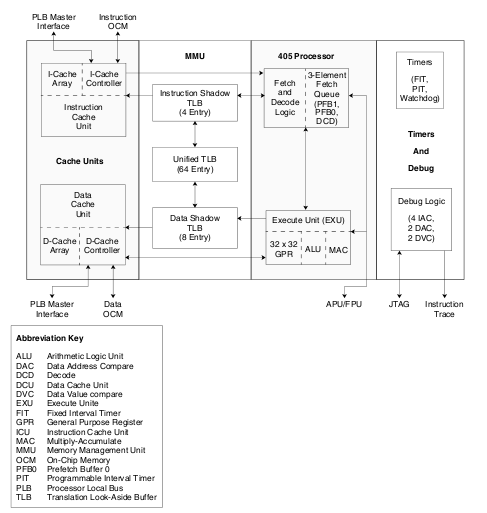
\includegraphics[scale=.60]{./figuras/arc_ppc405.png}
 % capas.png: 607x522 pixel, 72dpi, 21.41x18.41 cm, bb=0 0 607 522
 \caption{Organización del procesador \emph{PowerPC 405-S}}
 \label{Organización del procesador}
\end{figure}


\section{Compilación y carga del \emph{driver} en Linux}

Un controlador de dispositivo, llamado normalmente \emph{driver} es un programa
informático que permite al sistema operativo interactuar con un periférico,
haciendo una abstracción del hardware. Se puede esquematizar como un manual
de instrucciones que le indica al sistema operativo, cómo debe controlar y
comunicarse con un dispositivo en particular. Por tanto, es una pieza esencial,
sin la cual no se podría usar el hardware.

Debido a que el software de controladores de dispositivos se ejecuta como parte
del sistema operativo, con acceso sin restricciones a todo el equipo, resulta
esencial que sólo se permitan los controladores de dispositivos autorizados.

Los \emph{drivers} de la tarjeta de desarrollo NetFPGA se pueden obtener en la
siguiente dirección web:

\url{http://netfpga.org/foswiki/bin/view/NetFPGA/OneGig/Releases}

\subsection{Instalación de dependencias en Debian GNU/Linux}

Dependencia significa que un software necesita de otro para que funcione
adecuadamente. En Linux es común que se necesiten herramientas o librerías para
realizar un trabajo. Este problema se puede resolver, en parte, con programas
que se encargan del software instalado y que tratan de resolver las dependencias
con información proveída por personas encargadas de los paquetes.

En el caso de la tarjeta de desarrollo NetFPGA es necesaria la instalación de
dependencias en el sistema huesped con el fin de poder hacer la compilación del
código fuente del \emph{driver} de forma correcta.

A continuación se listan las dependencias requeridas en Debian GNU/Linux 6.0.4:

\begin{itemize}
 \item \textbf{libncurses5-dev}, este paquete contiene los archivos de
cabecera, bibliotecas estáticas y los enlaces simbólicos que los desarrolladores
que usan ncurses va a necesitar.\\

  \begin{verbatim}
  root@debian:~#apt-get install libncurses5-dev
  \end{verbatim}

 \item \textbf{libnet1-dev}, proporciona un marco portátil de paquete de red de
bajo nivel escritura y manipulación. libnet incluye las interfaces portátiles de
creación de paquetes en la capa IP y la capa de enlace, así como una gran
cantidad de funcionalidad adicional.

  \begin{verbatim}	
  root@debian:~\#apt-get install libnet1-dev
  \end{verbatim}

 \item \textbf{libpcap-dev}, proporciona un marco portátil de bajo nivel
red de monitoreo. Las aplicaciones incluyen estadísticas de la red
recolección, supervisión de la seguridad, la depuración de la red, etc.

  \begin{verbatim}	
  root@debian:~\#apt-get install libpcap-dev
  \end{verbatim}


\end{itemize}


\subsubsection{Compilación del \emph{driver}}

Se compila el \emph{driver}:

  \begin{verbatim}
  root@debian:~\#cd ~/netfpga/  make
  \end{verbatim}

Se instala el \emph{driver}:

  \begin{verbatim}
  root@debian:~#cd ~/netfpga/  make install >> salida_install.txt
  \end{verbatim}

Se reinicia el sistema:

  \begin{verbatim}
  root@debian:~#reboot
  \end{verbatim}

Una vez que el sistema a reiniciado se verifica la carga del \emph{driver}:

  \begin{verbatim}
  root@debian:~#lsmod  | grep nf2 
  nf2                    11925  0 
  \end{verbatim}


 \subsection{Instalación del \emph{driver} en CentOS }
  
Para hacer sencilla la instalación de los \emph{drivers}, se han creado 
paquetes \emph{RPM}\footnote{\emph{ RPM Package Manager} (o \emph{RPM},
originalmente llamado \emph{Red Hat Package Manager}) es una herramienta de
administración de paquetes pensada básicamente para \emph{GNU/Linux}. Es capaz
de instalar, actualizar, desinstalar, verificar y solicitar programas.
\emph{RPM} es el formato de paquete de partida del \emph{Linux Standard Base}.}
y un repositorio de \emph{YUM}\footnote{\emph{Yellow dog Updater, Modified} es
una herramienta libre de gestión de paquetes para sistemas \emph{Linux} basados
en \emph{RPM}.}. Se muestra a continuación los pasos a seguir para la
instalación de la tarjeta de desarrollo NetFPGA en sistemas CentOS y Fedora.

\begin{enumerate}
 \item Ingresar al sistema como usuario \emph{root}
   \begin{verbatim}
  [proyecto@CentOS ~]\$ su -
  Password: 
  [root@CentOS ~]#
  \end{verbatim}
  
 \item Instalar el repositorio \emph{RPMforge}
    \begin{verbatim}
  [root@CentOS ~]#rpm --import http://apt.sw.be/RPM-GPG-KEY.dag.txt
  \end{verbatim}
  
   \item Instalar el paquete descargado
    \begin{verbatim}
  [root@CentOS ~]#rpm -i rpmforge-release-0.5.2-2.el6.rf.*.rpm
  \end{verbatim}
  
     \item Instalar el  repositorio \emph{YUM} NetFPGA 
    \begin{verbatim}
  [root@CentOS ~]#rpm -Uhv
http://netfpga.org/yum/el5/RPMS/noarch/netfpga-repo-1-1_CentOS5.noarch.rpm 
  \end{verbatim}
  
       \item Instalar los paquetes base para la  NetFPGA 
    \begin{verbatim}
  [root@CentOS ~]#yum -y install netfpga-base
  \end{verbatim}
  
  \begin{itemize}
   \item NOTA: Es necesario instalar algunas dependencias para el correcto
funcionamiento de la tarjeta de desarrollo, YUM se encargará de instarlas
automáticamente durante este proceso.
  \end{itemize}  
\end{enumerate}

\subsubsection{Verificando la interfaces de la tarjeta de desarrollo NetFPGA}

Para comprobar que las cuatro interfaces \textbf{nf2cX} se han cargado
correctamente se utiliza el comando :

  \begin{verbatim}
  root@CentOS:~# ifconfig -a | grep nf2 
  nf2c0     Link encap:Ethernet  HWaddr 00:4e:46:32:43:00  
  nf2c1     Link encap:Ethernet  HWaddr 00:4e:46:32:43:01  
  nf2c2     Link encap:Ethernet  HWaddr 00:4e:46:32:43:02  
  nf2c3     Link encap:Ethernet  HWaddr 00:4e:46:32:43:03  
  \end{verbatim}

  
 \subsubsection{Reprogramando CPCI}
 
Una vez instalada la tarjeta de desarrollo en el sistema huesped se debe de
reprogramar el \emph{bus} \emph{CPCI} de la siguiente manera:

  \begin{verbatim}
  root@CentOS:~# /usr/local/sbin/cpci_reprogram.pl --all  
  \end{verbatim}
  
 Esperando la salida:
 
   \begin{verbatim}
   Loading the CPCI Reprogrammer on NetFPGA 0   
   Loading the CPCI on NetFPGA 0   
   CPCI on NetFPGA 0 has been successfully reprogrammed 
  \end{verbatim}
 
 Es necesario reprogramar el \emph{CPCI} cada vez que se inicie el sistema
huesped, esto se puede lograr de forma automatica agregando la siguiente liena
al archivo \emph{/etc/rc.local}:

   \begin{verbatim}
/usr/local/netfpga/lib/scripts/cpci_reprogram/cpci_reprogram.pl --all 
  \end{verbatim}
  

Con el fin de familiarizarse con la tarjeta de desarrollo durante la realizacón
del proyecto se realizaron varias pruebas con proyectos realizados
anteriormente por la comunidad de desarrolladores, estas pruebas se encuentran
documentadas en el \emph{Apéndice \ref{ApexB}}.             


% \section{XUPV5}

En este proyecto se usa la tarjeta Xilinx University Program Virtex 5 (XUPV5).
La tarjeta de desarrollo \emph{XUPV505} es un dispositivo con características
para la evaluación de proyectos de  propósito general, la plataforma de
desarrollo cuenta con memoria incrustrada e interfaces estándar de la industria
de conectividad. Cuenta con el dispositivo FPGA \emph{Virtex-5}.

\subsection{Características de la  tarjeta de desarrollo \emph{XUPV505} }

Las características con las que cuenta la tarjeta de desarrollo son:

\begin{itemize}
 \item FPGA Xilinx \emph{Virtex-5}  
 \item Dos Xilinx XCF32P Flash PROMs (32 Mbyte cada uno) para
configuraciones del dispositivo
 \item Xilinx SystemACE Compact Flash para configuraciones de control
 \item 64-bit 256Mbyte DDR2 small outline DIMM (SODIMM)
 \item 10/100/1000  Interfaces Ethernet 
 \item Intrefaz USB
 \item Sistema de reloj programable
 \item Puerto RS-232
\end{itemize}


\begin{figure}[h!]
 \centering
 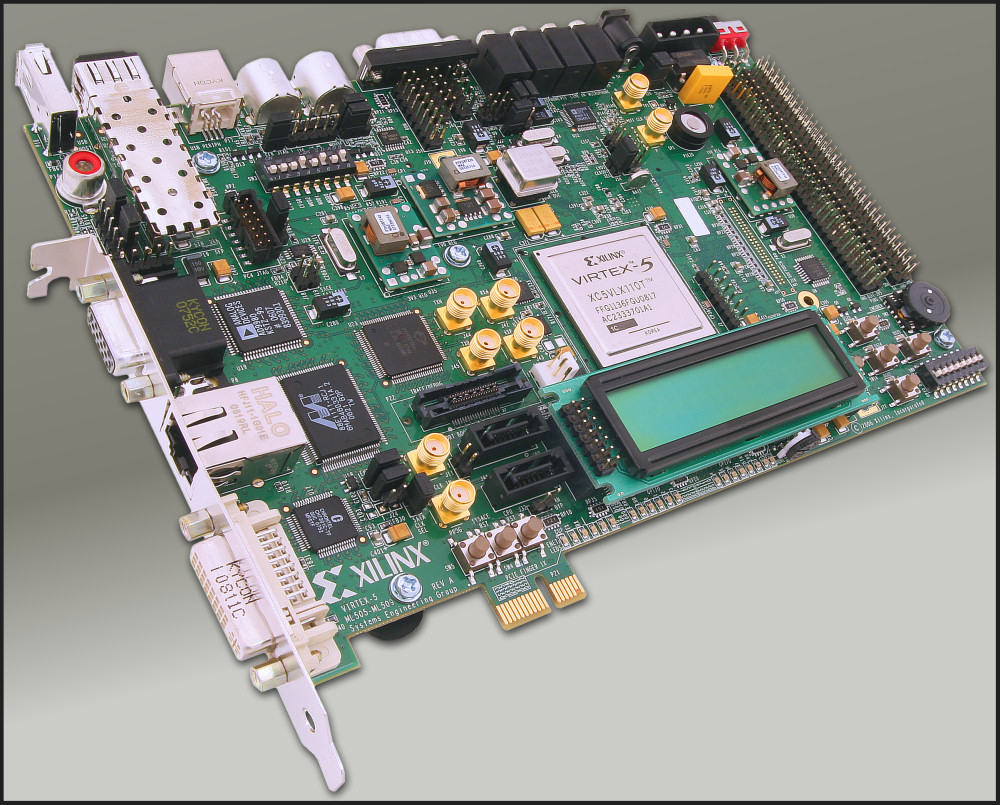
\includegraphics[scale=.30]{./figuras/V5.jpg}
 % V5.jpg: 1000x805 pixel, 72dpi, 35.28x28.40 cm, bb=0 0 1000 805
  \caption{Tarjeta de desarrollo XUPV505}
 \label{XUPV505}
\end{figure}

\section{XUPV2}

En este proyecto se usa la tarjeta Xilinx University Program Virtex 2 (XUPV2).
La tarjeta de desarrollo \emph{XUPV2} es un dispositivo con características
para la evaluación de proyectos de  propósito general, la plataforma de
desarrollo cuenta con memoria incrustrada e interfaces estándar de la industria
de conectividad. Cuenta con el dispositivo FPGA \emph{Virtex-2}.

\subsection{Características de la  tarjeta de desarrollo \emph{XUPV2} }

Las características con las que cuenta la tarjeta de desarrollo son:

\begin{itemize}
\item FPGA Virtex-2 Pro XC2VP30  con 30,816 celdas lógicas, 136 18-bit multiplicadores,
 2,448Kb bloques de RAM y 2 Procesadores PowerPC.
\item DDR SDRAM DIMM de hasta  2Gbytes de RAM
\item Puerto Ethernet 10/100
\item Puerto USB2 
\item Lector de tarjetas Compact Flash
\item Puerto de video XSGA
\item Audio Codec
\item Puertos SATA, S/2 y RS-232
\end{itemize}


\begin{figure}[h!]
 \centering
 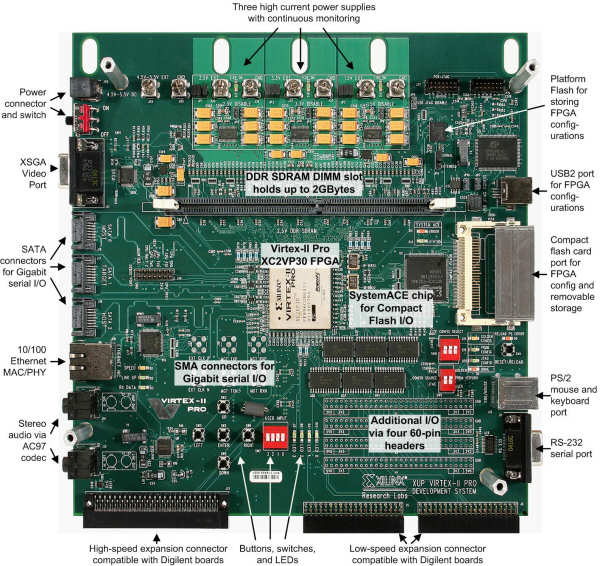
\includegraphics{./figuras/V2.jpg}
 % V5.jpg: 1000x805 pixel, 72dpi, 35.28x28.40 cm, bb=0 0 1000 805
  \caption{Tarjeta de desarrollo Virtex-II Pro Development System}
 \label{XUPV502}
\end{figure}


La lista detallada de características de la tarjeta de desarrollo \emph{XUPV2}
puede ser consultada en la dirección : 
\begin{center}
 \url{http://www.xilinx.com/univ/xupv2p.html}
\end{center}


 




